\documentclass{article}
\usepackage{graphicx}
\usepackage{amsmath}
\usepackage{pdfpages}

\begin{document}

\title{Monte Carlo, Session 2}
\author{Alexey Sofiev, 013573003}
\date{}
\maketitle

%\begin{abstract}
%The abstract text goes here.
%\end{abstract}

\section*{Exercise 1}
Ex1.cpp (run from main.cpp, to get the randoms.h connected correctly.)

The distribution obtained from LCG are presented in Figure \ref{fig:ex1lcg}.

\begin{figure}[!hbt]
	\includegraphics[width=350px]{"../Laskari2/ex1_lcg"}
	\caption{Ex1, LCG.}
	\label{fig:ex1lcg}
\end{figure}

The distribution obtained from PM are presented in Figure \ref{fig:ex1pm}.

\begin{figure}[!hbt]
	\includegraphics[width=350px]{"../Laskari2/ex1_pm"}
	\caption{Ex1, PM.}
	\label{fig:ex1pm}
\end{figure}

The distribution obtained from MT are presented in Figure \ref{fig:ex1mt}.

\begin{figure}[!hbt]
	\includegraphics[width=350px]{"../Laskari2/ex1_mt"}
	\caption{Ex1, MT.}
	\label{fig:ex1mt}
\end{figure}

Additionally, ex1.m produces that the average Chi2 value for LCG is 0.1525, for PM is 59.599 and for MT is 58.31. 

The degree of freedom is number of bins minus one, so it is 59 in our case. Then for $\alpha$=0.05 the lower tail is 39.662. PM and MT are bigger, but LCG fails since it is lower.


%\includepdf[pages={1}, scale=0.8]{Ex1.pdf}

\section*{Exercise 2}
Ex2.cpp

Generates data to subfolder data. N is $10^7$ and k is $10^6$.

At the start lets visualize all calculated $C_k$ values in Figure \ref{fig:ex2fig1}. 
\begin{figure}[!hbt]
	\includegraphics[width=350px]{"../Laskari2/ex2fig1"}
	\caption{Ex1, $C_k$ values from different generators}
	\label{fig:ex2fig1}
\end{figure}

As it can be seen, no too clear pattern observed, so lets take a look at histograms presented in Figure \ref{fig:ex2fig3}.


\begin{figure}[!hbt]
	\includegraphics[width=350px]{"../Laskari2/ex2fig3"}
	\caption{Ex1, abs($C_k$) values in histogram basing on generator.}
	\label{fig:ex2fig3}
\end{figure}

Theoretically, it is assumed to see rising around abs(x)=1 and lowering around 0. However, even due to usage of the course generators, onliest difference noticed is that LCG is more evenly distributed than the others.

\section*{Exercise 3}

The function is presented in Figure \ref{fig:ex3function}.
\begin{figure}[!hbt]
	\includegraphics[width=350px]{"../Laskari2/ex3function"}
	\caption{Ex3, the function.}
	\label{fig:ex3function}
\end{figure}
Basing on the image, the first box is when y is from 0 to 7. For the combined method lets use y from 0 to 3 while x from 0 to 4, and then the same y from 0 to 7 box.

Then, the program outputs the Figure \ref{fig:ex3result}. As it can be seen, the combined method is roughly twice better. (Better with smaller b, but becomes proportionally less effective when b>4, as it should according to definition)

\begin{figure}[!hbt]
	\includegraphics[width=250px]{"../Laskari2/ex3result"}
	\caption{Ex3, the result.the combined method is roughly twice better. Better with smaller b, but becomes proportionally less effective when b>4, as it should according to definition.}
	\label{fig:ex3result}
\end{figure}


\section*{Exercise 4}
\subsection*{Ex4, Inversion method}
\begin{equation}
	f(x)=\frac{10}{\pi \gamma}*\frac{\gamma^2}{x^2 + \gamma^2}, \ where \ \gamma =2
\end{equation}

\begin{equation}
	\int_{0}^{x}f(x)dx =\Big|_0^t \frac{10}{\pi \gamma} *\gamma *tan^{-1}\left(\frac{x}{\gamma}\right) = \frac{10}{\pi}*tan^{-1}\left(\frac{x}{\gamma}\right) =F(x)
\label{eq:Ex4F}
\end{equation}

Now lets check that F($\infty$) is 1.

\begin{equation}
	F(x\rightarrow\infty)=*...wolframalpha...*=\frac{10}{\pi}\frac{1}{2}\sqrt{\frac{1}{\gamma^2}}\gamma\pi =5
\end{equation}

Since we can produce random number from 0 to 1, we want F to be 1. Thus we scale the F function with $\pi/2$.

\begin{equation}
	s=\frac{F}{5}
\end{equation}

Now lets input F(x) from Equation \ref{eq:Ex4F}, and solve x as the function of s.

\begin{equation}
s=\frac{1}{5}*F=\frac{2}{\pi}*tan^{-1}\left(\frac{x}{\gamma}\right)
\end{equation}

\begin{equation}
	\Longrightarrow x=\gamma *tan\left( \frac{s*\pi}{2} \right)
\end{equation}\

And after setting the $\gamma =2$, we get:
\begin{equation}
	x=2 *tan\left( \frac{s*\pi}{2} \right)
\end{equation}
where s is the random value from 0 to 1.

To evaluate the result, random numbers are generated and presented as histogram in Figure \ref{fig:ex4histInv}. 
\begin{figure}[!hbt]
	\includegraphics[width=350px]{"../Laskari2/ex4histInv"}
	\caption{Histogram of random number that are generated using the inversion method.}
	\label{fig:ex4histInv}
\end{figure}

It can be noticed that the shape of Figure \ref{fig:ex4histInv} is similar as the wanted distribution formula presented in Figure \ref{fig:ex4Gaussian}.

Note: Additionally, limited acceptable x-values to range [-10,10] as were required in the task. 
Note: Due to periodicity of tan function the values from 0 to 10 and from 0 to -10 are generated similarly with only the sign difference.

\subsection*{Ex4, Combined method}

As suggested, lets simply try some Gaussian functions to be the upper function to presented f(x).

\begin{figure}[!hbt]
	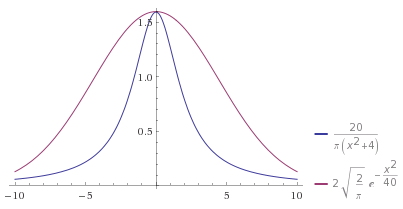
\includegraphics[width=350px]{../Laskari2/ex4Gaussian}
	\caption{Simple iteractive attempt to predict the suitable Gaussian.}
	\label{fig:ex4Gaussian}
\end{figure}

Basing on Figure \ref{fig:ex4Gaussian}, it can be concluded that g(x):

\begin{equation}
	g(x)=2*\sqrt{\frac{2}{\pi}}*e^{-\frac{x^2}{40}}
\end{equation}
is suitable for upper limit prediction.

Now lets do same operations, as done in the inversion method. This will allow to generate the random numbers according to upper distribution, which will lead to better hit-miss ratio.

To solve this, let's lead it to Box-Muller example presented in the lecture. Firstly, lets redefine:
\begin{equation}
	X=\frac{x}{\sqrt{20}}
\end{equation}
Now it is almost the example presented in the lecture, except that
\begin{equation}
	dX=\frac{dx}{\sqrt{20}}
\end{equation}

And on page 25 from Lecture 3, the
\begin{equation}
	f_\phi (\phi)=\frac{16}{2\pi}=\frac{8}{\pi}
\end{equation}

Therefore the task is to generate uniformly distributued $u_1$ and $u_2$. Then the angle can be obtained from:

\begin{equation}
	\phi = \frac{\pi}{8}u_1
\end{equation}
\begin{equation}
	r=\sqrt{-2 log(1-u_2)}
\end{equation}
\begin{equation}
	y=r*sin\phi
\end{equation}
\begin{equation}
	X=r*cos\phi
\end{equation}
\begin{equation}
	\Longrightarrow x=X*\sqrt{20}=\sqrt{20}*r* cos\phi
\end{equation}

This formulas result in Figure \ref{fig:ex4histComb}.
\begin{figure}[!hbt]
	\includegraphics[width=350px]{"../Laskari2/ex4histComb"}
	\caption{Histogram of random number that are generated using the combined method. (Gaussian with Box-Muller)}
	\label{fig:ex4histComb}
\end{figure}
Overall shape is suitable, but for some reason centered at 5. Thus it is possible to conclude that I am having a scalar error somewhere, not sure where.

\end{document}